\section{Boundary conditions}
\textbf{Start program}
To start the program you must be on a computer with the program on it. Then you just have to run the file. If you want the program to have the full functionality at synchronize the calendar, you must have a network connection. 
\newline
\newline
\textbf{Shutdown program}
To shut down the program you must be in the program, and be able to click on the lock down button. 
We have also clarified some boundary use cases that we have put in our use case diagram, to handle some different boundary exceptions. 


\begin{figure}[h]
\centering
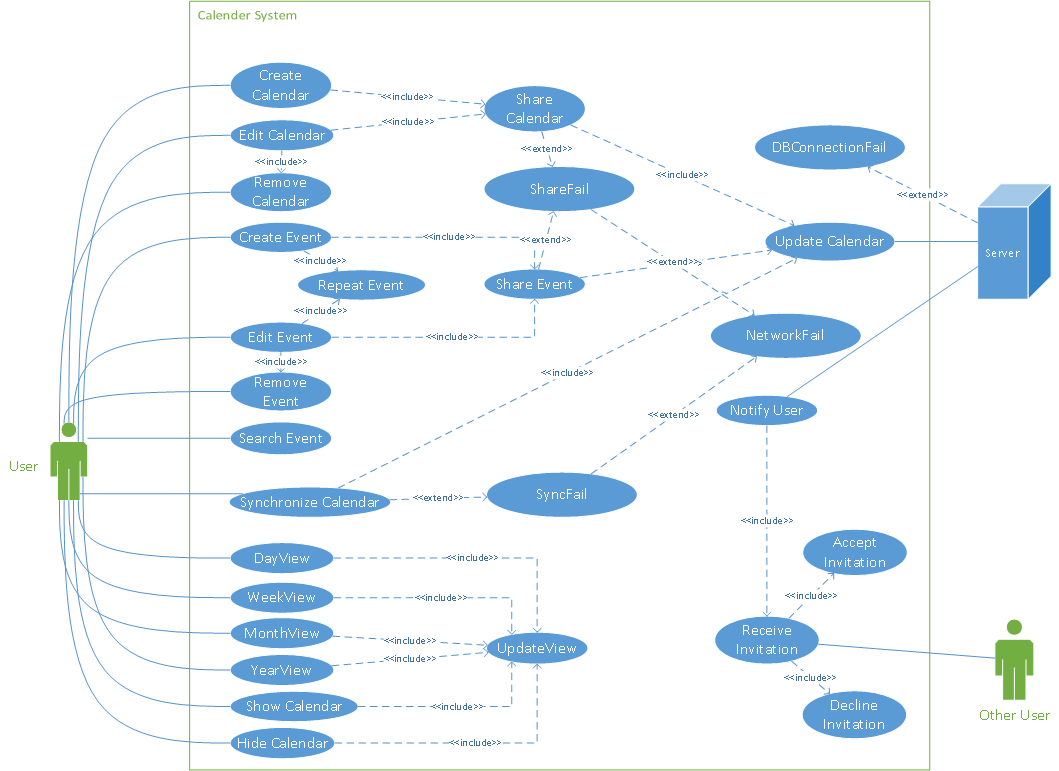
\includegraphics[width=160mm]{UMLUseCaseDiagram.png}
\caption{Updated UML Use Case diagram with  boundary conditions \label{overflow}}
\label{figur:usecase}
\end{figure}